% ------------------------------------------------------------------------------
% Copyright (c) 2019, 2022 Contributors to the Eclipse Foundation
%
% See the NOTICE file(s) distributed with this work for additional
% information regarding copyright ownership.
%
% This program and the accompanying materials are made available under the terms
% of the MIT License which is available at https://opensource.org/licenses/MIT
%
% SPDX-License-Identifier: MIT
% ------------------------------------------------------------------------------
\documentclass{article}
\usepackage{tikz}
\usepackage{verbatim}

\usepackage[paperwidth=40in, paperheight=20in]{geometry}

\usetikzlibrary{arrows, automata, positioning, shapes.misc}
\begin{document}
\pagestyle{empty}

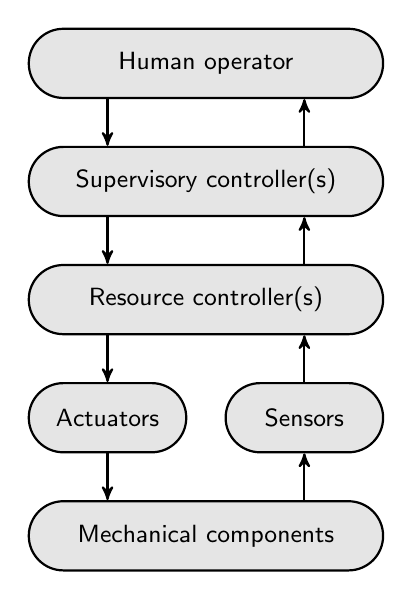
\begin{tikzpicture}[
  ->,>=stealth',auto,node distance=2.5cm,thick,
  every node/.style={font=\sffamily\small, inner sep=.25cm},
  every state/.style={fill=black!10,draw=black,thick,rounded rectangle},
  every edge/.style={draw=black}]

  \node[state, minimum width=5cm]   (hop) at (0cm,     6cm)   {Human operator};
  \node[state, minimum width=5cm]   (sup) at (0cm,     4.5cm) {Supervisory controller(s)};
  \node[state, minimum width=5cm]   (res) at (0cm,     3cm)   {Resource controller(s)};
  \node[state, minimum width=2.5cm] (act) at (-1.25cm, 1.5cm) {Actuators};
  \node[state, minimum width=2.5cm] (sen) at (1.25cm,  1.5cm) {Sensors};
  \node[state, minimum width=5cm]   (mch) at (0cm,     0cm)   {Mechanical components};

  \coordinate [left =1.25cm of hop.south] (hopSL);
  \coordinate [right=1.25cm of hop.south] (hopSR);
  \coordinate [left =1.25cm of sup.north] (supNL);
  \coordinate [right=1.25cm of sup.north] (supNR);
  \coordinate [left =1.25cm of sup.south] (supSL);
  \coordinate [right=1.25cm of sup.south] (supSR);
  \coordinate [left =1.25cm of res.north] (resNL);
  \coordinate [right=1.25cm of res.north] (resNR);

  \path[every node/.style={font=\sffamily\normalsize,outer sep=0pt}]
    (hopSL)                edge[] (supNL)
    (supSL)                edge[] (resNL)
    (res.south-|act.north) edge[] (act.north)
    (act.south)            edge[] (mch.north-|act.south)

    (supNR)                edge[] (hopSR)
    (resNR)                edge[] (supSR)
    (sen.north)            edge[] (res.south-|sen.north)
    (mch.north-|sen.south) edge[] (sen.south)
  ;

\end{tikzpicture}
\end{document}
